\section{Service discovery basics}
Recent advances in computer science make it possible to build small mobile devices with many features. They have a long battery lifetime, a powerful processor unit and can handle more and more advanced applications. Mobile devices are here not just Notebooks but also PDAs, mobile phones, MP3 Players and so on. Due to the growing abilities of mobile devices it became reasonable to connect them. The idea is to connect several mobile devices to a network to allow them to communicate with each other and to share their services. In this paper we want to observe the possibilities offered by service discovery protocol (SLP). We will compare its current weaknesses and create suggestions how to fix them. To begin with, we first introduce the usage of such mobile devices in an open network.\\
A possible scenario is for example a hotel where we can find several user groups. For hotel employees it would be useful if special hotel services would be multicast. Those services can be like ``available rooms", ``technical control", ``room cleaning" and so on. In this way a hotel employee has a possibility to be mobile and still make his work and controlling several hotel properties. Another user group could be the guests. For this group there are other useful services like ``room service", ``environment map", ``weather", ``great attractions" and so on. A guest would have a possibility to order something to his/her location (not necessarily into the room) or easily find out some interesting attractions near the hotel. But as both groups are in same network, there is also a need to hide and/or secure some services from unauthorized users. In case a vicious person gets access to the employee services he could control technical features or checking other guests in/out. Those problems should be prevented early. The guests shouldn't even be able to see the services for hotel employees and neither should they be able to use them. To hide the services and encrypt communication is already a way to prevent attacks on those services (more details will be discuss in section 3).\\
Other possible scenario is for example a person with a mobile phone who offers phone calls over an open network (we assume such a person has a national flat rate). Another person with a notebook could use such a service to call someone. Possible attackers could track the user and get the phone number he is calling or an attacker could betray the service provider with an international phone call. In this case it is reasonable to encrypt the communication between service provider and user and there should be a kind of trust that the service user doesn't use the service in a wrong way. But to make such an infrastructures work in this way there are some requirements to fulfill: 
\begin{itemize}
\item server and client have to be on the same network 
\item both should speak the same lingo (use same protocols for example) 
\item to use or provide sensitive services they need some kind of security to find services in the network 
\end{itemize}
The main subject of this paper is service discovery and its security issues that arise in hostile environment like open networks. This paper separates the service discovery and service invocation from each other and we don't discuss security issues after service invocation here. However, to understand the service discovery security and their weaknesses we first need to understand the basics of service providing and service discovery.\\

\subsection{Open network}
In this paper we are talking about networks as free or open networks. An open network is a network for everyone even for bad guys. It provides the possibility that everyone who wants to join this network will join it. In this way the network allows the communication between every peer that is a part of this network. Also the idea of an open network is to create a network everywhere without complicated operations. So the open network is very dynamical. The network can be created centralized with servers or it can be created decentralized with peer to peer communication. All peers can connect or disconnect to the network anytime and without any restrictions. In this way there are no constrains and you can connect every possible devices with each other like personal computers, servers, notebooks but also printers, mobile phones, mp3 players and other portable or stationary devices. Open networks aren't necessarily based on IPs but in this paper we work with service location protocol (SLP) so we presume the communication is IP based. How the open network works is not a part of this paper. Furthermore we don't treat security issues in open network itself and assume that it is secure \citep{Foundation2009}.

\subsection{Service discovery architecture}
There are three important architecture approaches used for service
discovery \citep{Ververidis2008}.

\subsubsection{Directory-based architecture}
In directory-based architecture network peers have three possibilities how they can act. A network peer can offer its services as SA (\textbf{s}ervice \textbf{a}gent) to other peers, it can use discovered services as UA (\textbf{u}ser \textbf{a}gent) and a network peer can act as DA (\textbf{d}irectory \textbf{a}gent) which caches services provided by other SAs and forwards them to user agents. Because an open network is a dynamic network it can't be assume that there is always a reachable directory agent. But it is also possible that more than just one DA is operating in an open network. A directory agent is an important instance in this architecture and is essential to keep the network alive. All devices (service agents) which want to provide their services have to register them by a directory agent.
They register their services by sending service description (e.g. service name, server IP, description what the service can do, etc.) to the directory agent which stores all that information. As soon as a user agent wants to use a service, it sends via unicast a request for a searched service to the DA or it request all services which the DA stores. After receiving the information about the requested service the UA can connect to the SA (also see figure 1.1). This architecture reduces the entire communication in the network. The devices don't need to communicate via multicast anymore, hence they don't force their resources which mean they also save battery lifetime. But on the other hand the benefit of this architecture is their biggest handicap at the same time. The DA in some kind centralizes the network and makes it vulnerable. If a DA leaves the network, the network also loses all the services that DA had stored. First problem arises for the SAs and UAs that they need a technique to notice a missing DA. And the other problem is that service providers and users have to find a new DA and for this time their services aren't reachable. In the worst-case they don't find a new DA and indirectly get excluded from the network. There are some approaches to avoid such cases but they aren't part of this paper so we won't discuss them here.

\begin{figure}[h]
\centering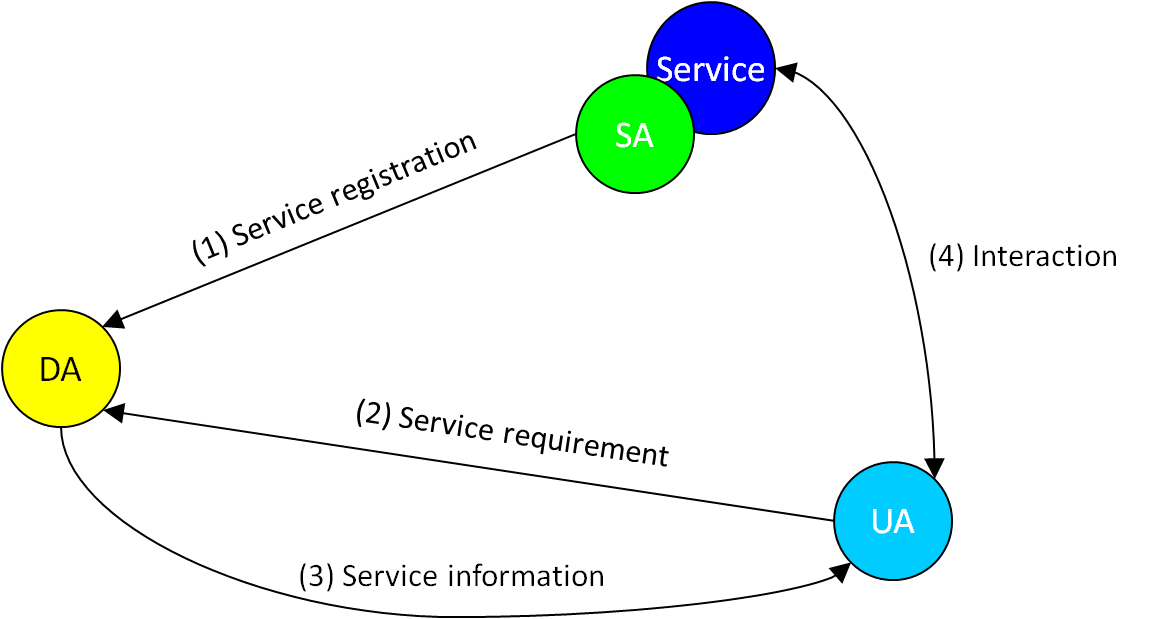
\includegraphics[width=0.5\textwidth]{Images/directory-based_architecture}
\caption{Directory-based architecture}
\end{figure}\noindent

\subsubsection{Directory-less architecture}
The directory-less architecture is quite contrary to the directory-based architecture. In this architecture the network peers can just act as service agents and as user agents. There is no directory agent so the service discovery should perform in other way. There are several approaches how this can be done. Service agents can distribute their services via multicast periodically send to the network. If a UA is interested in an offered service it requires the service information from the SA (also see figure 1.2). User agent can also discover services on their own by sending periodically a defined service request via multicast to the network till it gets an answer from a SA. Or a user agent can send a request to some network peers in its scope. In case a peer offers such a service it replies to the user agent otherwise the peer forwards the request to its neighbors and so on. In this architecture there is no central instance and it provides a much more stable network structure. However the communications via multicast drain more computation and battery lifetime from each network peer. Also to discover a service can take much longer compared to the directory-based architecture because there is no central authority that provides all services with their information.

\begin{figure}[h]
\centering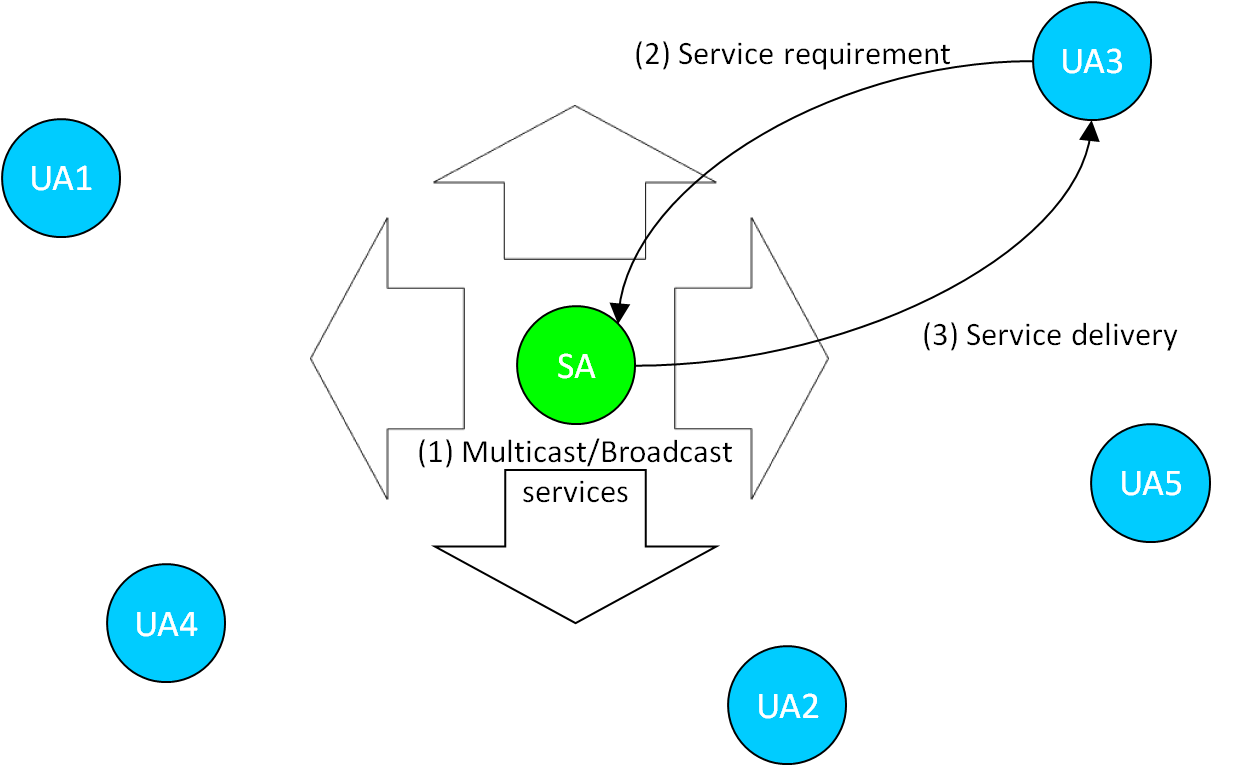
\includegraphics[width=0.5\textwidth]{Images/directory-less_architecture}
\caption{Directory-less architecture}
\end{figure}\noindent

\subsubsection{Hybrid architecture}
Hybrid architecture is a compromise of directory-based and directory-less architecture. Hybrid architecture combines the benefits of both other architectures. Like in directory-based architecture there are also three possibilities how a network peer can act (SA, UA and DA). To provide services a service agent first searches for a directory agent. In case a directory agent was found the service agent acts like in directory-based architecture and sends its service information to the DA and the DA is used by user agents to discover the services. In other case where no DA was located or all DAs left the network the SA acts like in directory-less architecture and periodically broadcast its services to the whole network. This architecture uses the benefits of the directory-based architecture to provide and discover services efficiently and to spare too many broad- and multicast communications in the network to keep battery lifetime from each network peer longer alive. At the same time the architecture offers a solution for the worst-case where no DAs are available in the network so the network won't die. The service location protocol, we will discuss below, is also based on the hybrid architecture.

\subsection{Secure service discovery basics}
Section 1.2 introduced some solutions how services can be provided and discovered in an open network. But there are also some security issues that prevent a secure usage of such a network. To safety use service discovery we have to fulfill at least the traditional security requirements:

\begin{itemize}
\item Authentication 
\item Authorization 
\item Integrity 
\item Confidentiality 
\end{itemize}
\citet{Cotroneo2004} suggests securing the registration and deregistration of the services. If a service is to be registered/deregistered it is important that authentication, authorization, integrity and confidentiality are maintained. In that way only authorized service agents can register or deregister their services. While registering a service, the communication has to be secured (by encryption) to prevent changes in the transferred information (integrity and confidentiality). With these common techniques many attacks like replay attack, user tracking or manipulating service information can already be prevented or become at least difficult (see also following sections). But just to secure the registration and deregistration is not enough. After the service discovery phase a user agent and service agent need an authentication between each other to keep their trust. Only authorized network peers should access the registered services. Authentication is needed in first way for the service agent who gets the information that the service was delivered to the right node if authentication was successful. And if a service agent authenticates itself by the user agent, user agent can be sure to trust the delivered service. Specific techniques to solve this problem are for example ``Web of Trust" and ``Public Key Infrastructure" which will be discussed in section 3.1.\\
Another important feature is the availability. It is not a secure issue in a first way but a network should also be able to detect broken service providers and delete them from the services list to prevent possible exploitations.